\section{Building NWAs from other NWAs (or ``the \texttt{wali::nwa::construct} namespace'')}
\label{Se:Building NWAs}

NWAs do not need to be built state-by-state and transition-by-transition;
they can also be built by performing language-theoretic operations upon
other NWAs. The supported operations are union, intersection, concatenation,
reversal, Kleene star, complement, and determinization.

The library supports two interfaces to each of these functions. In one, the
operation allocates an NWA with \texttt{new}, performs the construction, and
returns a \texttt{NWARefPtr} to the result.  In the other, the operation takes
a reference to an NWA, clears it, and constructs the result in-place.

Each of these functions is in the namespace \texttt{wali::nwa::construct}:

\begin{description}

  \item\texttt{NWARefPtr unionNWA( NWA const \& a, NWA const \& b )}
  \item\texttt{void unionNWA( NWA \& out, NWA const \& a, NWA const \& b )}
    Computes the union of the NWAs \texttt{a} and \texttt{b},
    either returning the result or storing it in \texttt{out}.
    See Section
    \ref{Se:Union}.

  \item\texttt{NWARefPtr intersect( NWA const \& a, NWA const \& b )}
  \item\texttt{void intersect( NWA \& out, NWA const \& a, NWA const \& b )}
    Computes the intersection of the NWAs \texttt{a} and \texttt{b},
    either returning the result or storing it in \texttt{out}.
    See Section \ref{Se:Intersection}.

  \item\texttt{NWARefPtr concat( NWA const \& left, NWA const \& right )}
  \item\texttt{void concat( NWA \& out, NWA const \& left, NWA const \& right )}
    Computes the concatenation of the NWAs \texttt{left} and
    \texttt{right}, either returning the result or storing it in
    \texttt{out}.
    See Section \ref{Se:Concatenation}.

  \item\texttt{NWARefPtr star( NWA const \& orig )}
  \item\texttt{void star( NWA \& out, NWA const \& orig )}
    Computes the Kleene-Star of the NWA \texttt{orig}, either
    returning the result or storing it in \texttt{out}. See Section
    \ref{Se:Star}.

  \item\texttt{NWARefPtr reverse( NWA const \& orig )}
  \item\texttt{void reverse( NWA \& out, NWA const \& orig )}
    Computes the NWA which accepts the reverse of each nested word
    accepted by the NWA \texttt{orig}, either returning the result or
    storing it in \textt{out}. See Section \ref{Se:Reverse}.

  \item\texttt{NWARefPtr determinize( NWA const \& orig )}
  \item\texttt{NWARefPtr determinize( NWA \& out, NWA const \& orig )}
    Computes a determinization of \texttt{orig}, either returning the
    result or storing it in \texttt{out}.
    See Section \ref{Se:Determinize}.

  \item\texttt{NWARefPtr complement( NWA const \& orig )}
  \item\texttt{void complement( NWA \& out, NWA const \& orig )}
    Computes the complement of the determinization of \texttt{orig},
    either returning the result or storing it in \texttt{out}.
    See Section
    \ref{Se:Complement}.
\end{description}

\subsection{Union}
\label{Se:Union}
Consider an example of computing the union of two NWAs, the NWA shown in
Figure \ref{Fig:Example1} and the NWA shown in Figure \ref{Fig:Union1}.  The
union of the NWAs is constructed by taking the component-wise union. (In
particular, it does \textsl{not} do the cross-product construction, and will
\textsl{always} produce a nondeterministic automaton as a result as long as
both machines have at least one initial state.)
The NWA resulting from the union of the
NWA shown in Figure \ref{Fig:Example1} and the NWA shown in Figure
\ref{Fig:Union1} is shown in Figure \ref{Fig:Union2}.

\begin{figure}[htbp]
  \centering
    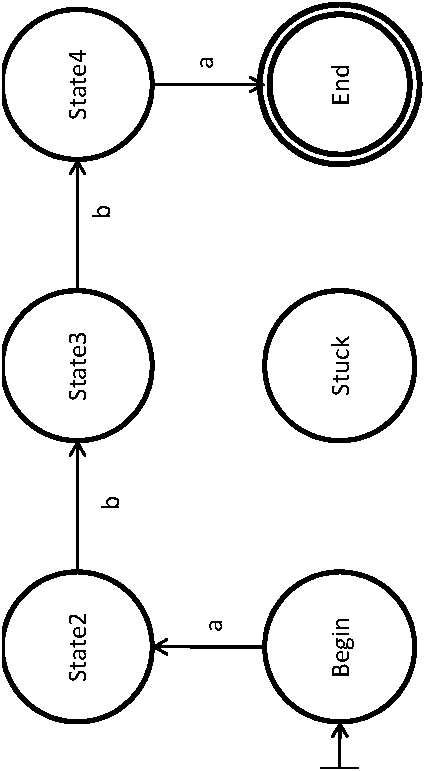
\includegraphics[width=8cm]{Figures/Figure3}
  \caption{Simple NWA to union with the NWA in Figure \ref{Fig:Example1}.}
  \label{Fig:Union1}
\end{figure}

\begin{figure}[htbp]
  \centering
    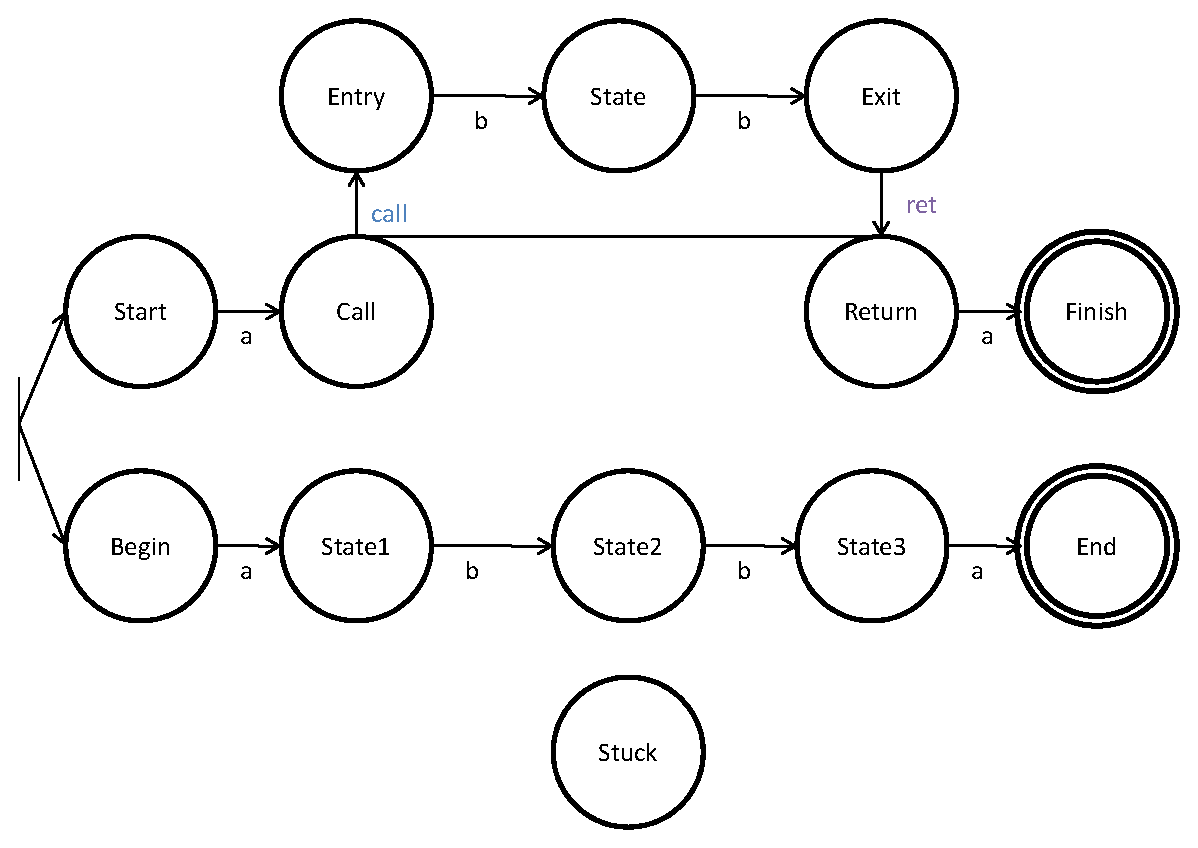
\includegraphics[width=12cm]{Figures/Figure4}
  \caption{The NWA resulting from the union of the NWA in Figure
    \ref{Fig:Example1} and the NWA in Figure \ref{Fig:Union1}.}
  \label{Fig:Union2}
\end{figure}

To construct the union of two
NWAs, the state sets of the NWAs cannot overlap,
i.e. $Q_1 \cap Q_2 = \emptyset$. \textsl{Client code should not depend on
  this condition being checked} or any particular behavior occurring if it
does not hold. (Currently the condition is checked in an assertion.)

Client information is copied directly from the original NWAs using
\texttt{ClientInfo::clone()}.


\subsection{Intersection}
\label{Se:Intersection}

The intersection of two NWAs is computed in the standard cross-product
fashion, except using a worklist algorithm to only compute those states that
are reachable.

The intersection is constructed by traversing the original NWAs starting at
the initial states and incrementally adding transitions for each pair of
``intersectable'' transitions that are encountered. By default, transitions
are ``intersectable'' when the transitions are the same kind (internal, call,
or return) and the symbols on the edge are identical (or at least one is wild
or epsilon).

The resulting NWA is shown in
Figure \ref{Fig:Intersect2}.
 
\begin{figure}[htbp]
  \centering
    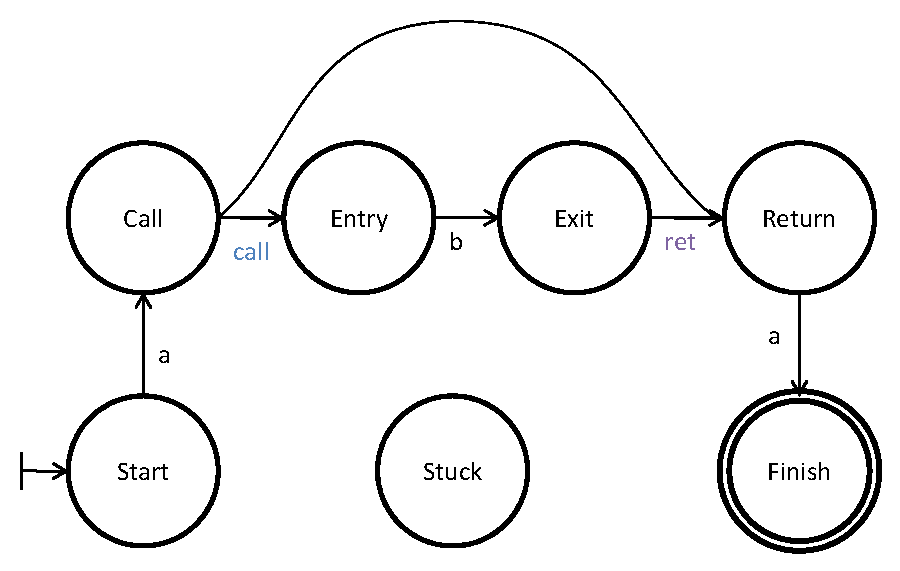
\includegraphics[width=10cm]{Figures/Figure5}
  \caption{Simple NWA to intersect with the NWA in Figure \ref{Fig:Example1}.}
  \label{Fig:Intersect1}
\end{figure}

\begin{figure}[htbp]
  \centering
    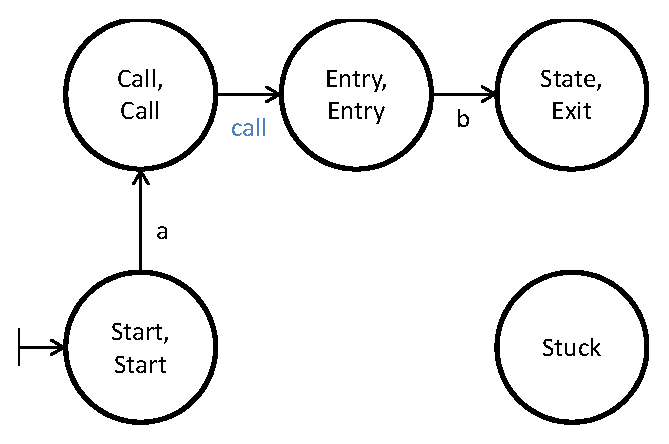
\includegraphics[width=8cm]{Figures/Figure6}
  \caption{The NWA resulting from the intersection of the NWA in Figure
    \ref{Fig:Example1} and the NWA in Figure \ref{Fig:Intersect1}.}
  \label{Fig:Intersect2}
\end{figure}

It is possible to customize what symbols are considered equivalent by
overriding the \texttt{transitionIntersect} function in a subclass of
\texttt{NWA}. In addition, it is possible to impose additional constraints on
what states can be combined by overriding \texttt{stateIntersect}. Both
functions also produce the result of the intersection:
\texttt{transitionIntersect} produces the symbol that will be used on the
resulting edge, and \texttt{stateIntersect} produces the state that will be
used as the target.

The default behavior of
\texttt{transitionIntersect} is that two transitions are intersectable if
neither symbol is epsilon and either the symbols are the same or at least one of
the symbols is a wild. (Epsilon transitions are dealt with in
\texttt{intersect} itself. If you override \texttt{transitionIntersect}, it
should return \texttt{false} if either input is epsilon.)

The default behavior of \texttt{stateIntersect} is that any two
states can be combined, the resulting state is labeled with a
\texttt{Key} that is uniquely generated from the pair of the \texttt{Keys} of
the two states under consideration, and the client information associated
with the resulting state is \texttt{null}.


Client information is generated by the helper method \texttt{stateIntersect},
but can be altered through the use of the helper methods
\texttt{intersectClientInfoInternal}, \texttt{intersectClientInfoCall}, and
\texttt{intersect\-Client\-InfoReturn}, which are invoked by
\texttt{intersect} as transitions of the three different kinds involving the
associated state are added.  The default behavior of these three functions is
to perform no changes to the \texttt{ClientInfo}.  These methods can be
overridden in subclasses to specify alternative behaviors.

\goodbreak
\noindent The following operations are methods of class NWA and are intended
to be overridden to customize behavior:

\begin{description}

  \item\texttt{bool stateIntersect( NWA const \& first, Key state1,\\ 
                   \hspace*{3.25cm} NWA const \& second, Key state2,\\
                   \hspace*{3.25cm} Key\& resSt, ref\_ptr<ClientInfo>\& resCI )}
    \nopagebreak

    Determines whether the given states can be combined and,
    if so, creates the combined state. If the two states are incompatable,
    returns \texttt{false}. If the two states are compatable, it computes the
    key of the combined state (storing it in \texttt{resSt} and the client
    information (storing it in \texttt{resCI}), then returns \texttt{true}.

  \item\texttt{bool transitionIntersect( NWA const \& first, Key
    sym1,\\ \hspace*{3.25cm} NWA const \& second, Key
    sym2,\\ \hspace*{3.25cm} Key\& resSym )} \nopagebreak

    Determines whether the given symbols are considered to be equivalent for
    the purposes of intersection. If so, it computes the symbol which should
    be associated with the combined transition (storing it in
    \texttt{resSym}) and returns true. If not, returns false.

  \item\texttt{void intersectClientInfoInternal( \\ \hspace*{3.25cm}
    NWA const \& first, Key src1, Key tgt1,\\ \hspace*{3.25cm} NWA const \&
    second, Key src2, Key tgt2,\\ \hspace*{3.25cm} Key resSym, Key resSt )}
    \nopagebreak

    Alters the client information associated with \texttt{resSt} given the
    sources and targets (as well as access to the client information
    associated with each state) of the two internal transitions that are
    being intersected.

  \item\texttt{void intersectClientInfoCall( \\ \hspace*{3.25cm}
    NWA const \& first ,Key call1, Key entry1,\\ \hspace*{3.25cm}
    NWA const \& second, Key call2, Key entry2,\\ \hspace*{3.25cm} Key
    resSym, Key resSt )} \nopagebreak

    Alters the client information associated with \texttt{resSt} given the
    call sites and entry points (as well as access to the client information
    associated with each state) of the two call transitions that are being
    intersected.

  \item\texttt{void intersectClientInfoReturn( \\ \hspace*{1.75cm}
    NWA const \& first, Key exit1, Key call1, Key ret1,\\ \hspace*{1.75cm}
    NWA const \& second, Key exit2, Key call2, Key ret2,\\ \hspace*{1.75cm}
    Key resSym, Key resSt )} \nopagebreak

    Alters the client information assoicated with \texttt{resSt} given the
    exit point, call site, and return site (as well as access to the client
    information associated with each state) of the two return transitions
    that are being intersected. \\

\end{description}


Consider the slightly more complex example of computing the intersection of
the NWAs shown in Figure \ref{Fig:Intersect3}.  The resulting NWA is shown in
Figure \ref{Fig:Intersect4}.

\begin{figure}[p]
  \centering
    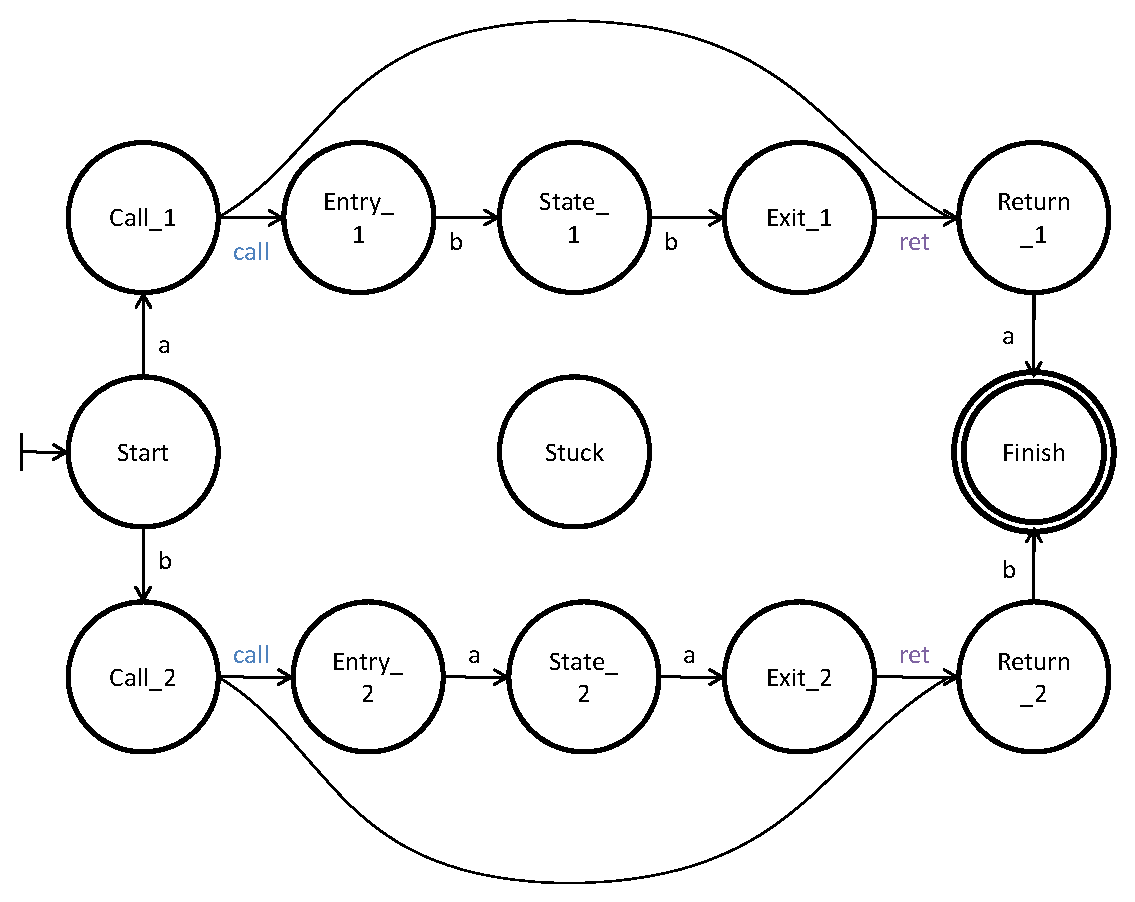
\includegraphics[width=12cm]{Figures/Figure7a}
    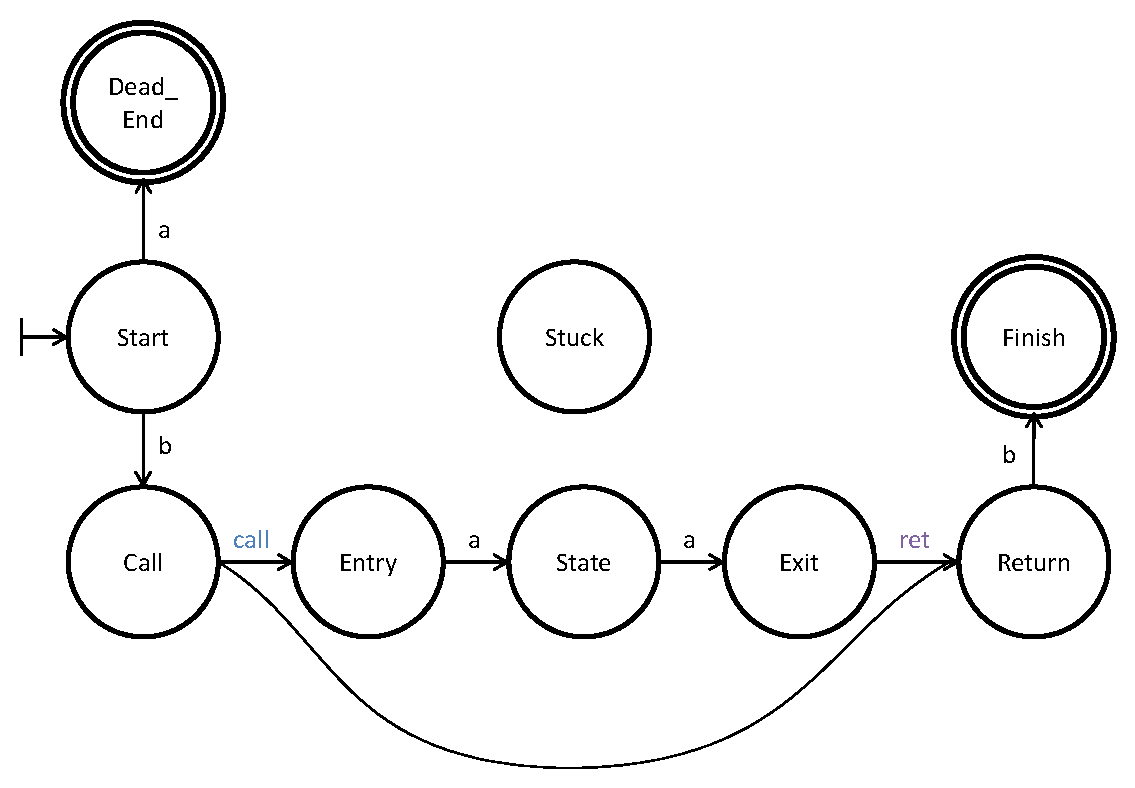
\includegraphics[width=12cm]{Figures/Figure7b}
  \caption{Complex NWAs to intersect.}
  \label{Fig:Intersect3}
\end{figure}

\begin{figure}[p]
  \centering
    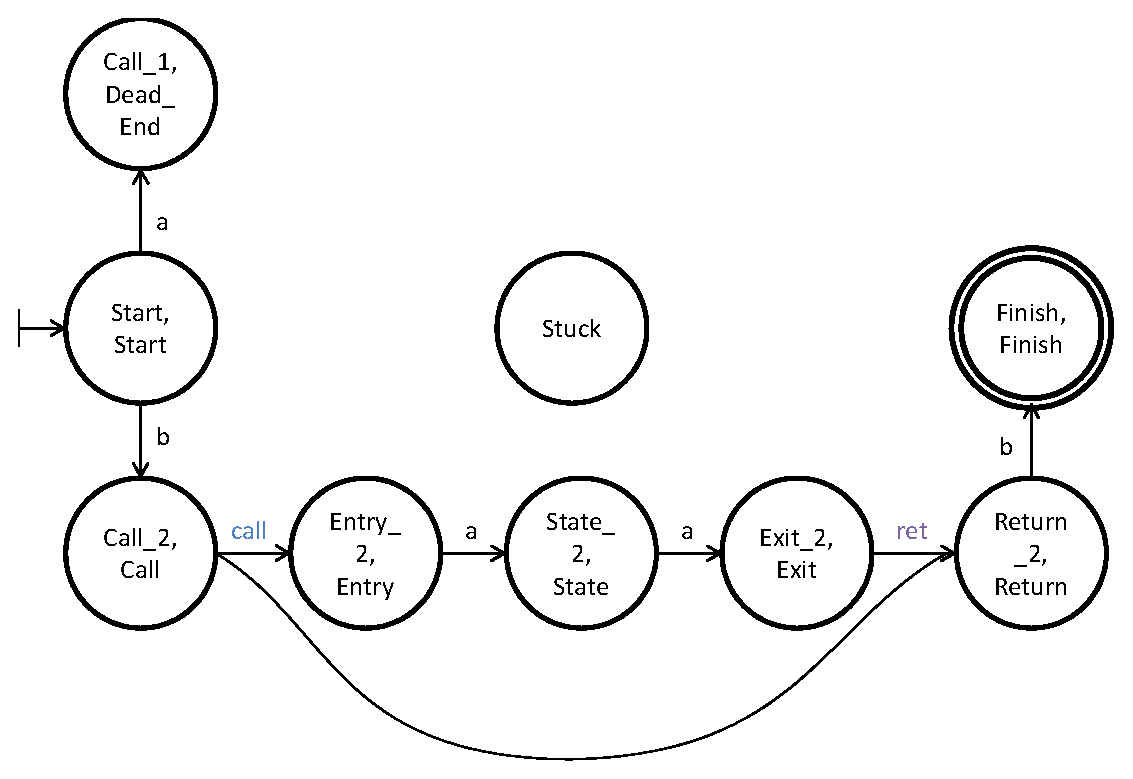
\includegraphics[width=12cm]{Figures/Figure8}
  \caption{The NWA resulting from the intersection of the NWAs in Figure \ref{Fig:Intersect3}.}
  \label{Fig:Intersect4}
\end{figure}



\subsection{Concatenation}
\label{Se:Concatenation}

Consider an example of computing the concatenation of two NWAs, the NWA shown
in Figure \ref{Fig:Example1} and the NWA shown in Figure \ref{Fig:Concat1}.
The concatenation is constructed by combining all states and transitions of
the first NWA (shown in Figure \ref{Fig:Example1}) and all states and
transitions of the second NWA (shown in Figure \ref{Fig:Concat1}) then adding
internal epsilon transitions from each final state of the first NWA to each
initial state of the second NWA.  In the resulting NWA, the initial states
are the initial states from the first NWA; the final states are the final
states of the second NWA.  If the original NWAs are $(Q_1, \Sigma_1,
{Q_0}_1, \delta_1, {Q_f}_1)$ and $(Q_2, \Sigma_2, {Q_0}_2, \delta_2,
{Q_f}_2)$, then the resulting NWA is $(Q, \Sigma, Q_0, \delta, Q_f)$ where $Q
= Q_1 \cup Q_2$, $\Sigma = \Sigma_1 \cup \Sigma_2$, $Q_0 = {Q_0}_1$, $\delta
= \delta_1 \cup \delta_2 \cup \delta_\epsilon$ (where $\delta_\epsilon =
\{(q,\epsilon,q') | q \in {Q_f}_1, q' \in {Q_0}_2\}$, and $Q_f = {Q_f}_2$ .
The NWA resulting from the concatenation of the NWA in Figure
\ref{Fig:Example1} and the NWA shown in Figure \ref{Fig:Concat1} is shown in
Figure \ref{Fig:Concat2}.

In
order to construct the concatenation of two NWAs, the state sets of the NWAs
cannot overlap, i.e. $Q_1 \cap Q_2 = \emptyset$
Client information is copied directly from the original NWAs using
\texttt{ClientInfo::clone()}.


\begin{figure}[p]
  \centering
    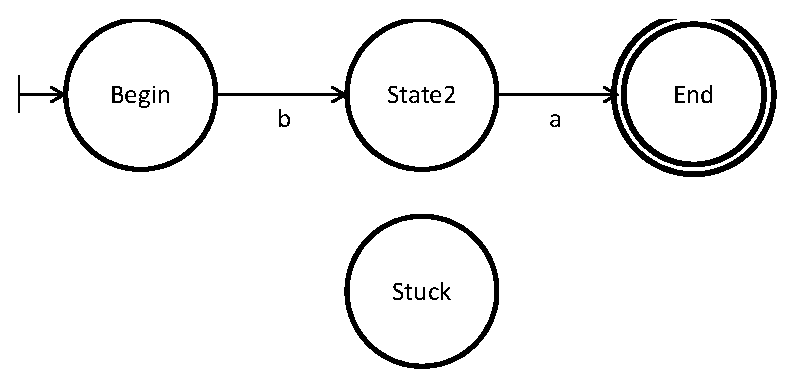
\includegraphics[width=10cm]{Figures/Figure9}
  \caption{Simple NWA to concatenate onto the NWA in Figure \ref{Fig:Example1}.}
  \label{Fig:Concat1}
\end{figure}

\begin{figure}[p]
  \centering
    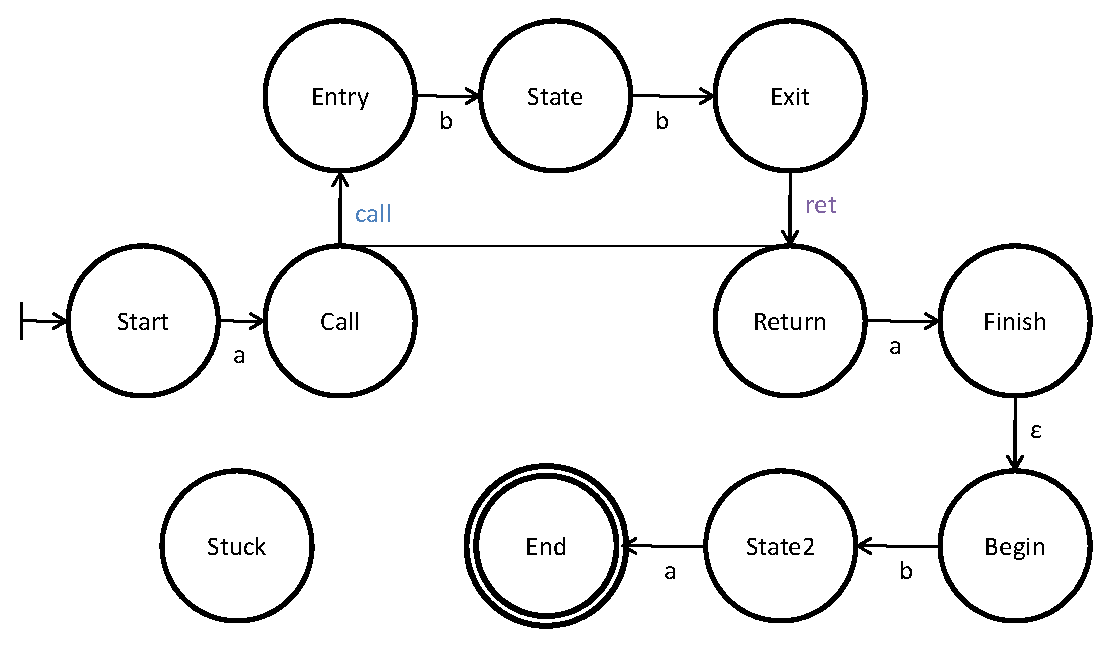
\includegraphics[width=12cm]{Figures/Figure10}
  \caption{The NWA resulting from the concatenation of the NWA in Figure
    \ref{Fig:Example1} with the NWA in Figure \ref{Fig:Concat1}.}
  \label{Fig:Concat2}
\end{figure}


\subsection{Kleene-Star}
\label{Se:Star}

Consider an example of computing the Kleene-Star of the NWA shown in Figure
\ref{Fig:Star1}.  If the original NWA is $(Q, \Sigma, Q_0, \delta, Q_f)$,
then the result of performing Kleene-Star on that NWA is $(Q \cup Q', \Sigma,
Q_0', \delta', Q_0')$ where $Q' = \{q' | q \in Q\}$ and $\delta' =
\{\delta_i',\delta_c',\delta_r'\}$ such that

\begin{enumerate} 

\item For all $(q,a,p) \in \delta_i$, the result NWA has $(q,a,p) \in
  \delta_i'$ and $(q',a,p') \in \delta_i'$, and if $p \in Q_f$, then
  $(q,a,r') \in \delta_i'$ and $(q',a,r') \in \delta_i'$ for each $r \in
  Q_0$,

\item For all $(q,a,p) \in \delta_c$, the result NWA has $(q,a,p) \in
  \delta_c'$ and $(q',a,p) \in \delta_c'$, and if $p \in Q_f$, then $(q,a,r')
  \in \delta_c'$ and $(q',a,r') \in \delta_c'$ for each $r \in Q_0$,

\item For all $(q,r,a,p) \in \delta_r$, the result NWA has $(q,r,a,p) \in
  \delta_r'$ and $(q,r',a,p') \in \delta_r'$, and if $p \in Q_f$, then
  $(q,r,a,s') \in \delta_r'$ and $(q,r',a,s') \in \delta_r'$ for each $s \in
  Q_0$, and

\item For all $(q,r,a,p) \in \delta_r$ with $r \in Q_0$, the result NWA has
  $(q',s,a,p') \in \delta_r'$ for each $s \in Q \cup Q'$, and if $p \in Q_f$,
  then $(q',s,a,t') \in \delta_r'$ for each $s \in Q \cup Q'$ and $t \in Q_0$

\end{enumerate}  

\noindent The NWA resulting from performing Kleene-Star on the NWA shown in
Figure \ref{Fig:Star1} is shown in Figure \ref{Fig:Star2}.  Note: The primed
states, $q'$ are constructed using \texttt{getKey($q$,getKey(prime))} where
$q \in Q$ and \texttt{prime} is the string ``prime''.

\begin{figure}[p]
  \centering
    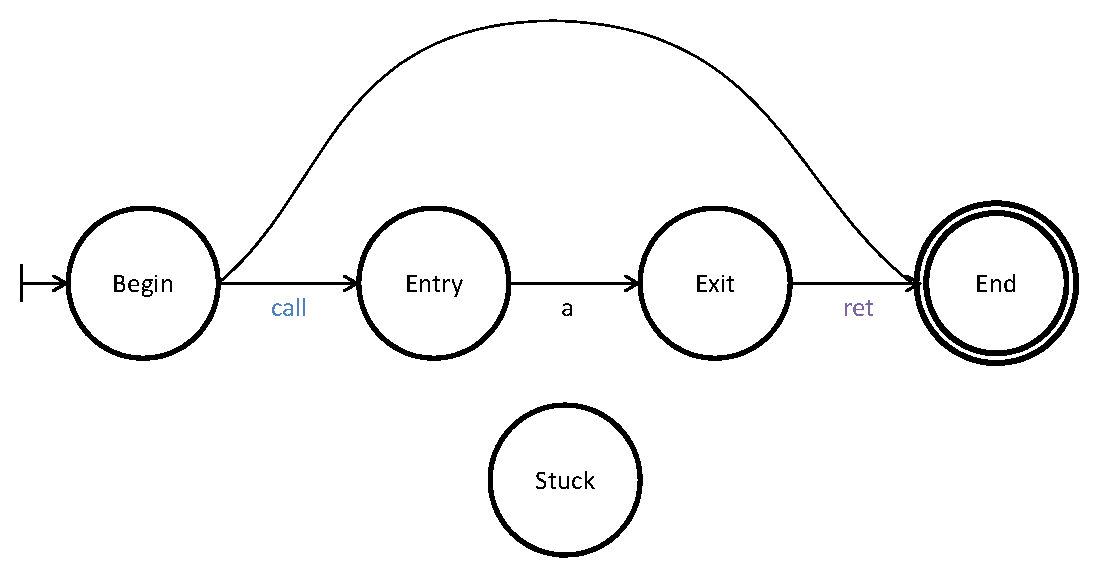
\includegraphics[width=10cm]{Figures/Figure11}
  \caption{An NWA on which to perform Kleene-Star.}
  \label{Fig:Star1}
\end{figure}

\begin{figure}[p]
  \centering
    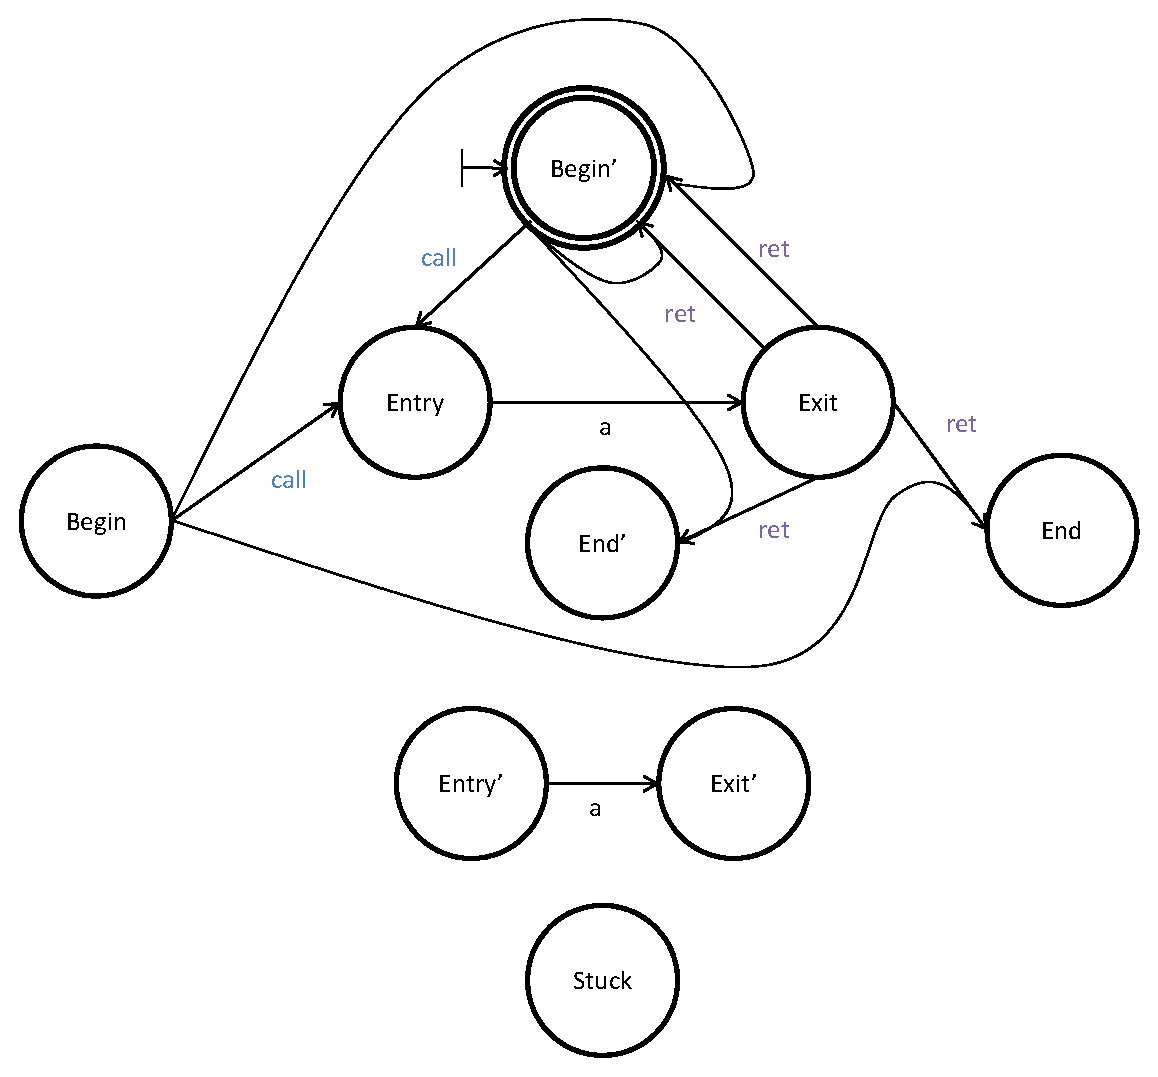
\includegraphics[width=12cm]{Figures/Figure12}
  \caption{The NWA resulting from performing Kleene-Star on the NWA in Figure \ref{Fig:Star1}.}
  \label{Fig:Star2}
\end{figure}

\goodbreak Client information is copied directly from the original NWA (using
\texttt{ClientInfo::clone()}) such that for each $q \in Q$, $q$
and $q'$ have the same client information.

%Consider the slightly more complex example of computing the Kleene-Star of the NWA shown in Figure \ref{Fig:Star3}.  The resulting NWA is shown in Figure \ref{Fig:Star4}.

%\begin{figure}[htbp]
%  \centering
%    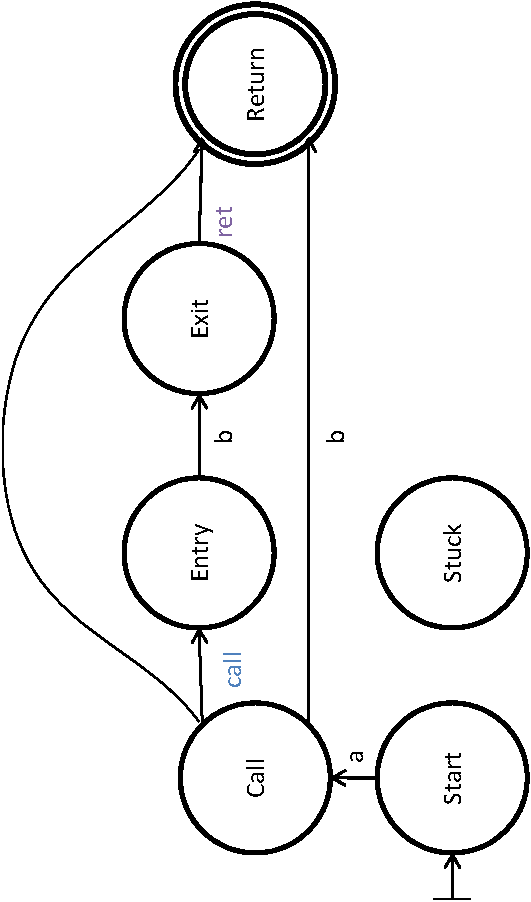
\includegraphics[angle=270,width=10cm]{Figures/Figure13.pdf}
%  \caption{Complex NWA on which to perform Kleene-Star.}
%  \label{Fig:Star3}
%\end{figure}

%\begin{figure}[htbp]
%  \centering
%    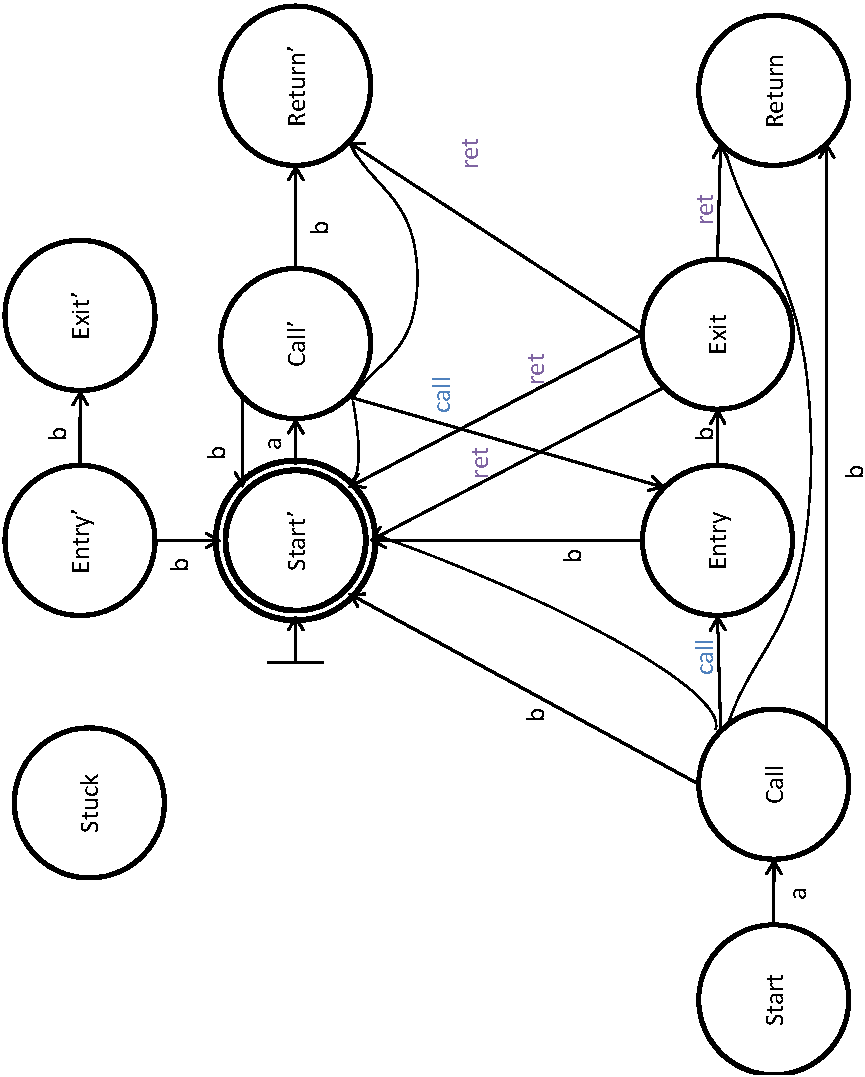
\includegraphics[angle=270,width=12cm]{Figures/Figure14.pdf}
%  \caption{The NWA resulting from performing Kleene-Star on the NWA in Figure \ref{Fig:Star3}.}
%  \label{Fig:Star4}
%\end{figure}

\subsection{Reverse}
\label{Se:Reverse}

If the original NWA is $(Q, \Sigma, Q_0, \delta, Q_f)$, then the result of
reversing that NWA is $(Q, \Sigma, Q_0, \delta_{rev}, Q_f)$ such that

\begin{enumerate}

\item For all $(q,\sigma,q') \in \delta_i$, the result NWA has $(q',\sigma,q)
  \in {\delta_{rev}}_i$

\item For all $(q_c,\sigma,q_e) \in \delta_c$, the result NWA has
  $(q_e,\sigma,q_c) \in {\delta_{rev}}_c$

\item For all $(q_x,q_c,\sigma,q_r) \in \delta_r$ and $(q_c,\sigma,q_e) \in
  \delta_c$ (where the $q_c$s are the same), the result NWA has
  $(q_r,q_e,\sigma,q_x) \in {\delta_{rev}}_r$

\end{enumerate}

\noindent The NWA resulting from performing reverse on the NWA shown in
Figure \ref{Fig:Example1} is shown in Figure \ref{Fig:Reverse1}.
 
\begin{figure}[p]
  \centering
    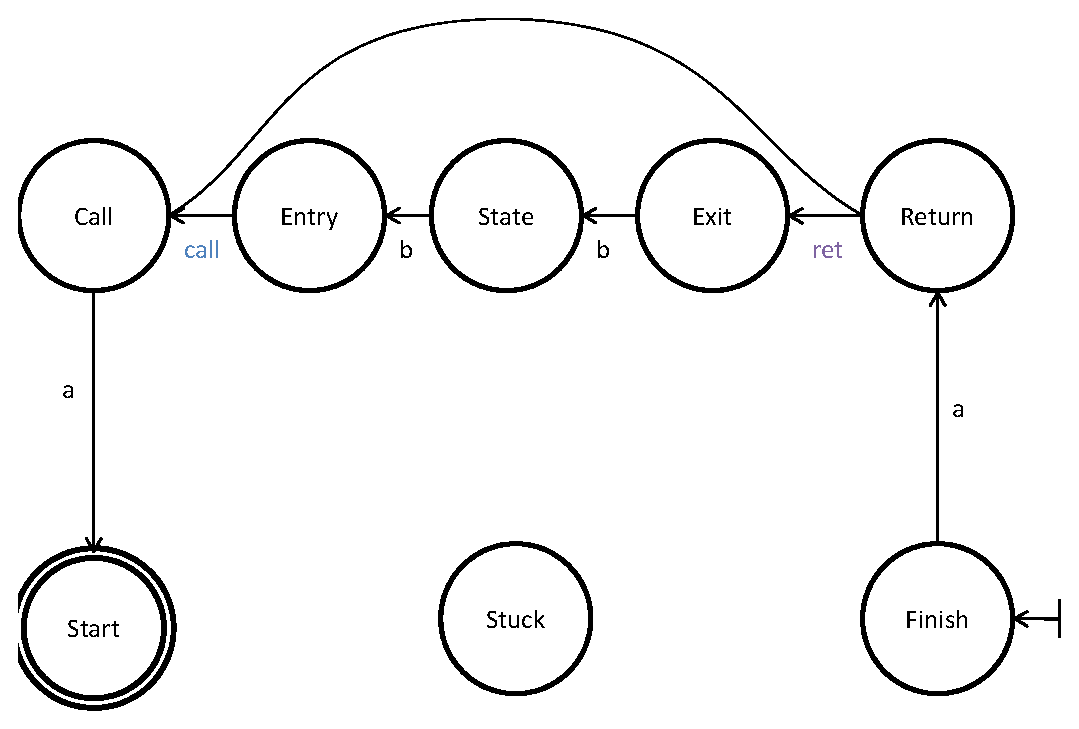
\includegraphics[width=12cm]{Figures/Figure15}
  \caption{The NWA resulting from performing reverse on the NWA in Figure \ref{Fig:Example1}.}
  \label{Fig:Reverse1}
\end{figure}

Client
information is copied directly from the original NWA using
\texttt{ClientInfo::clone()}.

\subsection{Determinize}
\label{Se:Determinize}

\begin{definition}
An NWA, $(Q,\Sigma,Q_0,\delta,Q_f)$, is \textbf{deterministic} iff 

\begin{enumerate} 

\item $|Q_0| = 1$, 

\item For all $q \in Q$: 
  \begin{itemize}
    \item if $(q,*,q') \in \delta_i$ then $|\{q'|(q,\sigma,q') \in
      \delta_i\}| = 0$; otherwise, for all $\sigma \in \Sigma - \{*\},
      |\{q'|(q,\sigma,q') \in \delta_i\}| \leq 1$,

    \item if $(q,*,q') \in \delta_c$ then $ |\{q'|(q,\sigma,q') \in
      \delta_c\}| = 0$; otherwise for all $\sigma \in \Sigma - \{*\},
      |\{q'|(q,\sigma,q') \in \delta_c\}| \leq 1$, and

    \item for all $q' \in Q$, if $(q,q',*,q'') \in \delta_r$ then
      $|\{q''|(q,q',\sigma,q'') \in \delta_r\}| = 0$; otherwise for all
      $\sigma \in \Sigma - \{*\}, |\{q''|(q,q',\sigma,q'') \in \delta_r\}|
      \leq 1$, and
  \end{itemize}
\item For all $(q,\sigma,q') \in \delta_i, \sigma \neq \epsilon$,

 for all $(q,\sigma,q') \in \delta_c, \sigma \neq \epsilon$,  and 

 for all $(q,q',\sigma,q'') \in \delta_r, \sigma \neq \epsilon$.\\

\end{enumerate}

If an NWA is not deterministic, then it is \textbf{non-deterministic}.
\end{definition}

Consider an example of determinizing a simple nondeterministic NWA, the NWA
shown in Figure \ref{Fig:Det1}.  The deterministic NWA is computed by a
generalization of the classical subset construction.  Instead of the states
in the determinized NWA being subsets of the original NWA, states of the
determinized NWA are sets of state pairs (i.e., binary relations on states)
\cite{JACM:AM2009}.  To support determinization, the library provides class
\texttt{BinaryRelation}, which is a set of \texttt{Key} pairs.  The resulting
NWA is shown in Figure \ref{Fig:Det2}.

\begin{figure}[p]
  \centering
    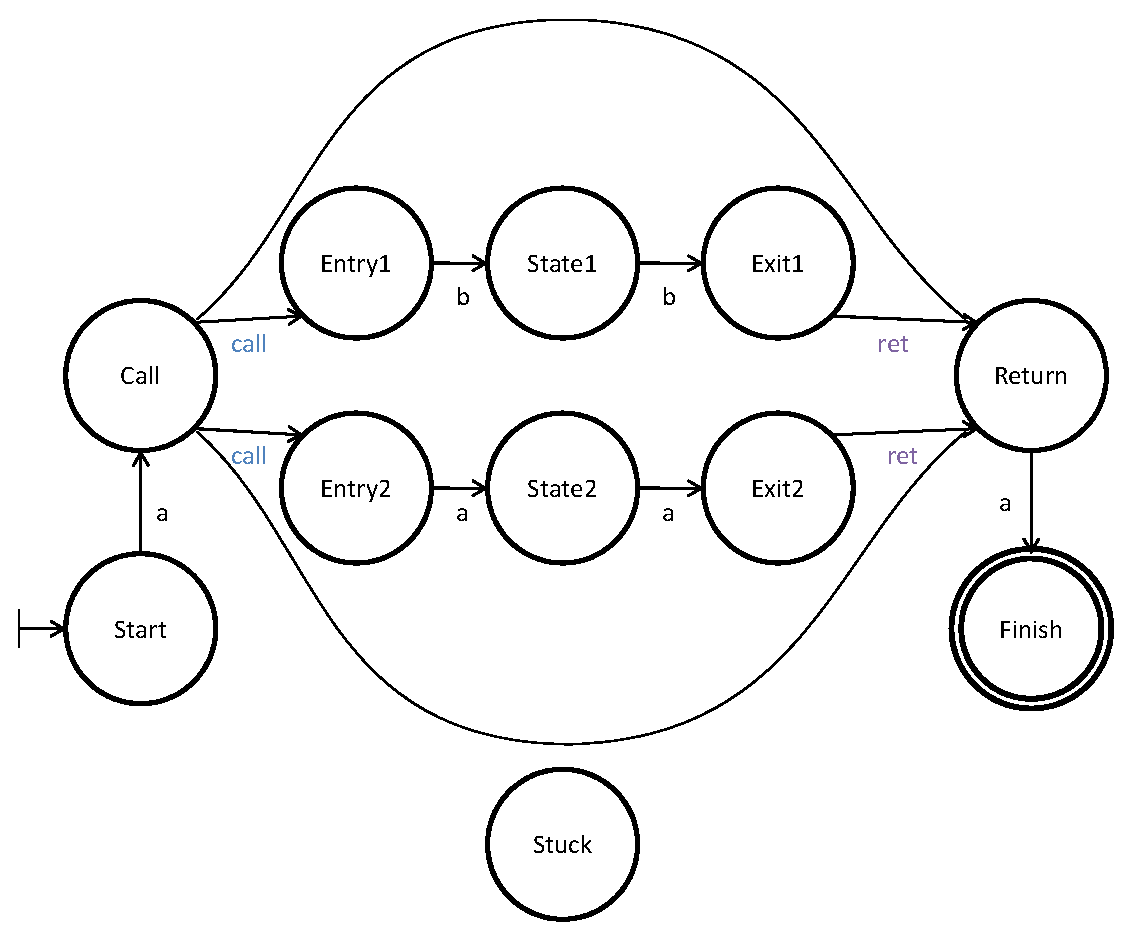
\includegraphics[width=12cm]{Figures/Figure16}
  \caption{Simple nondeterministic NWA.}
  \label{Fig:Det1}
\end{figure}


\begin{figure}[p]
  \centering
    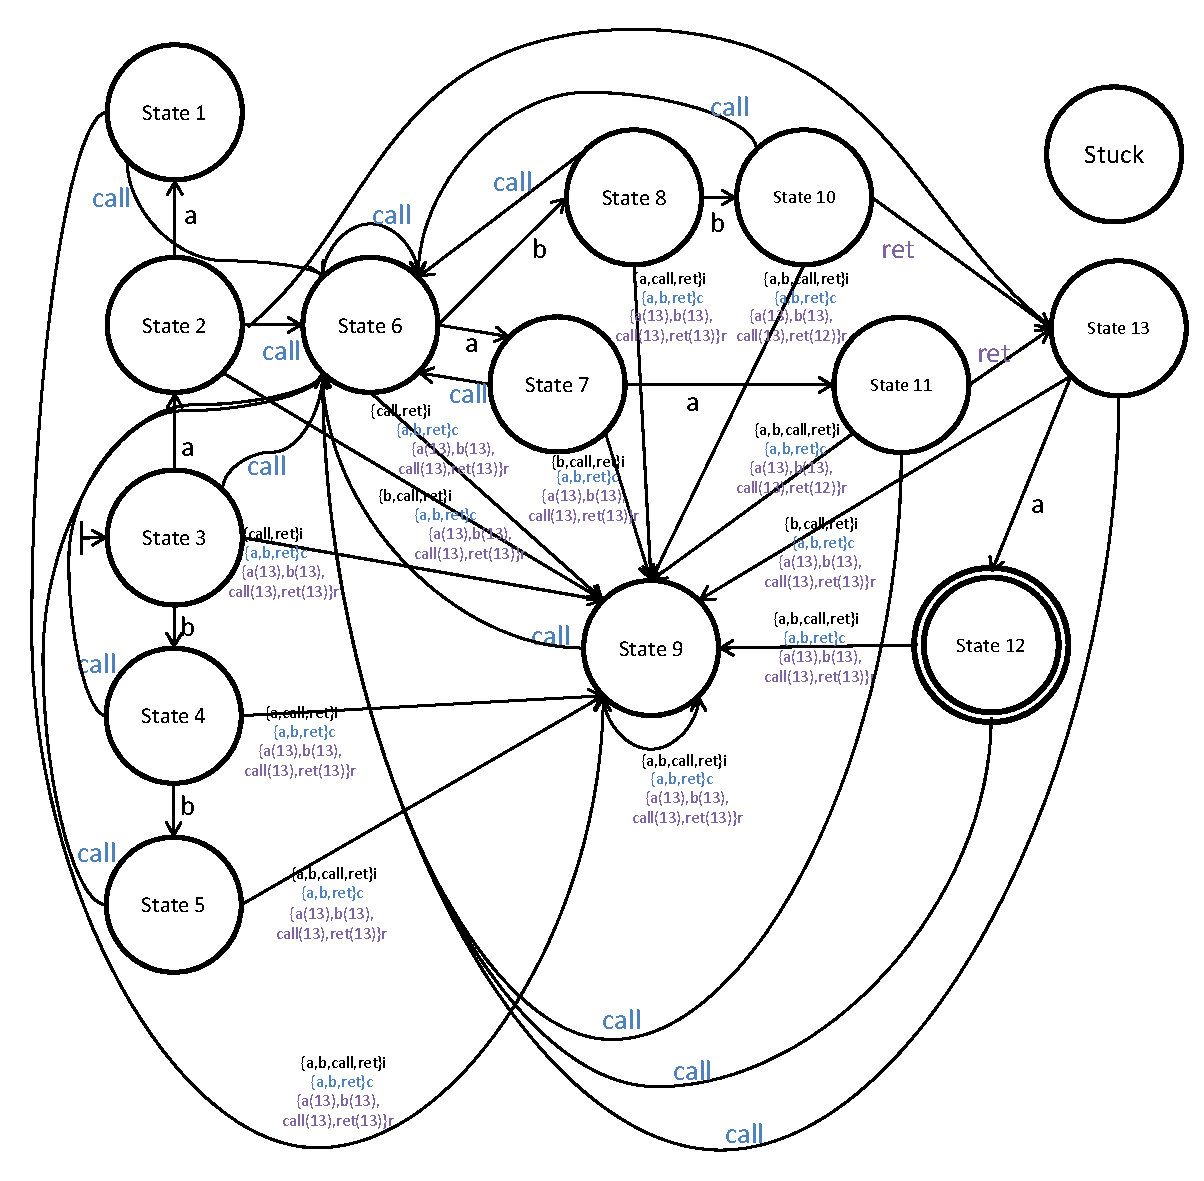
\includegraphics[width=16cm]{Figures/Figure17}
    \caption{The NWA resulting from determinizing the NWA in Figure
      \ref{Fig:Det1}. As mentioned in the text, states in the determinized
      NWA are relations on the states in the original NWA. For example, state
      1 above corresponds to the relation $\{$(Start,Stuck), (Call,Stuck),
      (Entry1,Stuck), (Entry2,Exit2), (State1,Stuck), (State2,Stuck),
      (Exit1,Stuck), (Exit2,Stuck), (Return,Stuck), (Fishish,Stuck),
      (Stuck,Stuck)$\}$.}
 
  \label{Fig:Det2}
\end{figure}


Client information is generated through the use of the helper method
\texttt{mergeClientInfo}, but can be altered through the use of the helper
methods \texttt{mergeClientInfoInternal}, \texttt{mergeClientInfoCall}, and
\texttt{mergeClientInfoReturn}, which are invoked by \texttt{determinize} as
transitions of the three kinds involving the associated state are added.  The
default behavior of \texttt{mergeClientInfo} is that the \texttt{ClientInfo}
associated with the resulting state is \texttt{null}.  The default behavior
of \texttt{mergeClientInfoInternal}, \texttt{mergeClientInfoCall}, and
\texttt{mergeClientInfoReturn} is to make no changes to the the
\texttt{ClientInfo}.  These methods can be overridden to specify alternative
behaviors.  As determinization is performed, \texttt{mergeClientInfo} is
called each time a new state is created.  Then, as each transition is added,
\texttt{mergeClientInfoInternal}, \texttt{mergeClientInfoCall}, or
\texttt{mergeClientInfoReturn} is called (depending on the type of transition
being added) to update the \texttt{ClientInfo} associated with the target
state of the transition being added. \\

\noindent The following operations are methods of class NWA and are intended
to be overridden to customize behavior:

\begin{description}

  \item\texttt{void mergeClientInfo( NWA const \& first,\\ \hspace*{3.25cm}
    BinaryRelation const\& binRel,\\ \hspace*{3.25cm} St resSt,
    ref\_ptr<ClientInfo>\& resCI )} \nopagebreak

    Computes the client information that should be associated with the given state.

  \item\texttt{void mergeClientInfoInternal( NWA const \& first,\nopagebreak
    \\ \hspace*{3.25cm} BinaryRelation const\& binRelSource,\nopagebreak
    \\ \hspace*{3.25cm} BinaryRelation const\& binRelTarget, \nopagebreak
    \\ \hspace*{3.25cm} Key sourceSt, Key resSym, Key resSt, \nopagebreak
    \\ \hspace*{3.25cm} ref\_ptr<ClientInfo>\& resCI )} \nopagebreak

    Alters the client information associated with \texttt{resSt} given the
    details of the internal transition to be added to the NWA.

  \item\texttt{void mergeClientInfoCall( NWA const \&
    first,\\ \hspace*{3.25cm} BinaryRelation const\&
    binRelCall,\\ \hspace*{3.25cm} BinaryRelation const\&
    binRelEntry,\\ \hspace*{3.25cm} Key callSt, Key resSym, Key
    resSt,\\ \hspace*{3.25cm} ref\_ptr<ClientInfo>\& resCI )} \nopagebreak

    Alters the client information associated with \texttt{resSt} given the
    details of the call transition to be added to the NWA.

  \item\texttt{void mergeClientInfoReturn( NWA const \&
    first,\\ \hspace*{3.25cm} BinaryRelation const\&
    binRelExit,\\ \hspace*{3.25cm} BinaryRelation const\&
    binRelCall,\\ \hspace*{3.25cm} BinaryRelation const\&
    binRelReturn,\\ \hspace*{3.25cm} Key exitSt, Key callSt, Key
    resSym,\\ \hspace*{3.25cm} Key resSt, ref\_ptr<ClientInfo>\& resCI )}
    \nopagebreak

    Alters the client information associated with \texttt{resSt} given the
    details of the return transition to be added to the NWA. \\

\end{description}

%Consider the slightly more complex determinization of the NWA shown in Figure \ref{Fig:Det3}.  The resulting NWA is shown in Figure \ref{Fig:Det4}.

%\begin{figure}[htbp]
%  \centering
%    \includegraphics[angle=270,width=12cm]{Figures/Figure18.pdf}
%  \caption{Complex nondeterministic NWA.}
%  \label{Fig:Det3}
%\end{figure}

%\begin{figure}[htbp]
%  \centering
%    \includegraphics[angle=270,width=12cm]{Figures/Figure19.pdf}
%  \caption{The NWA resulting from determinizing the NWA in Figure \ref{Fig:Det3}.}
%  \label{Fig:Det4}
%\end{figure}

\subsection{Complement}
\label{Se:Complement}

The complement is performed by first determinizing the NWA and then
complementing the final-state set of the determinized NWA.  The NWA resulting
from performing the complement of the NWA shown in Figure \ref{Fig:Det1} is
shown in Figure \ref{Fig:Comp1}.

\begin{figure}[p]
  \centering
    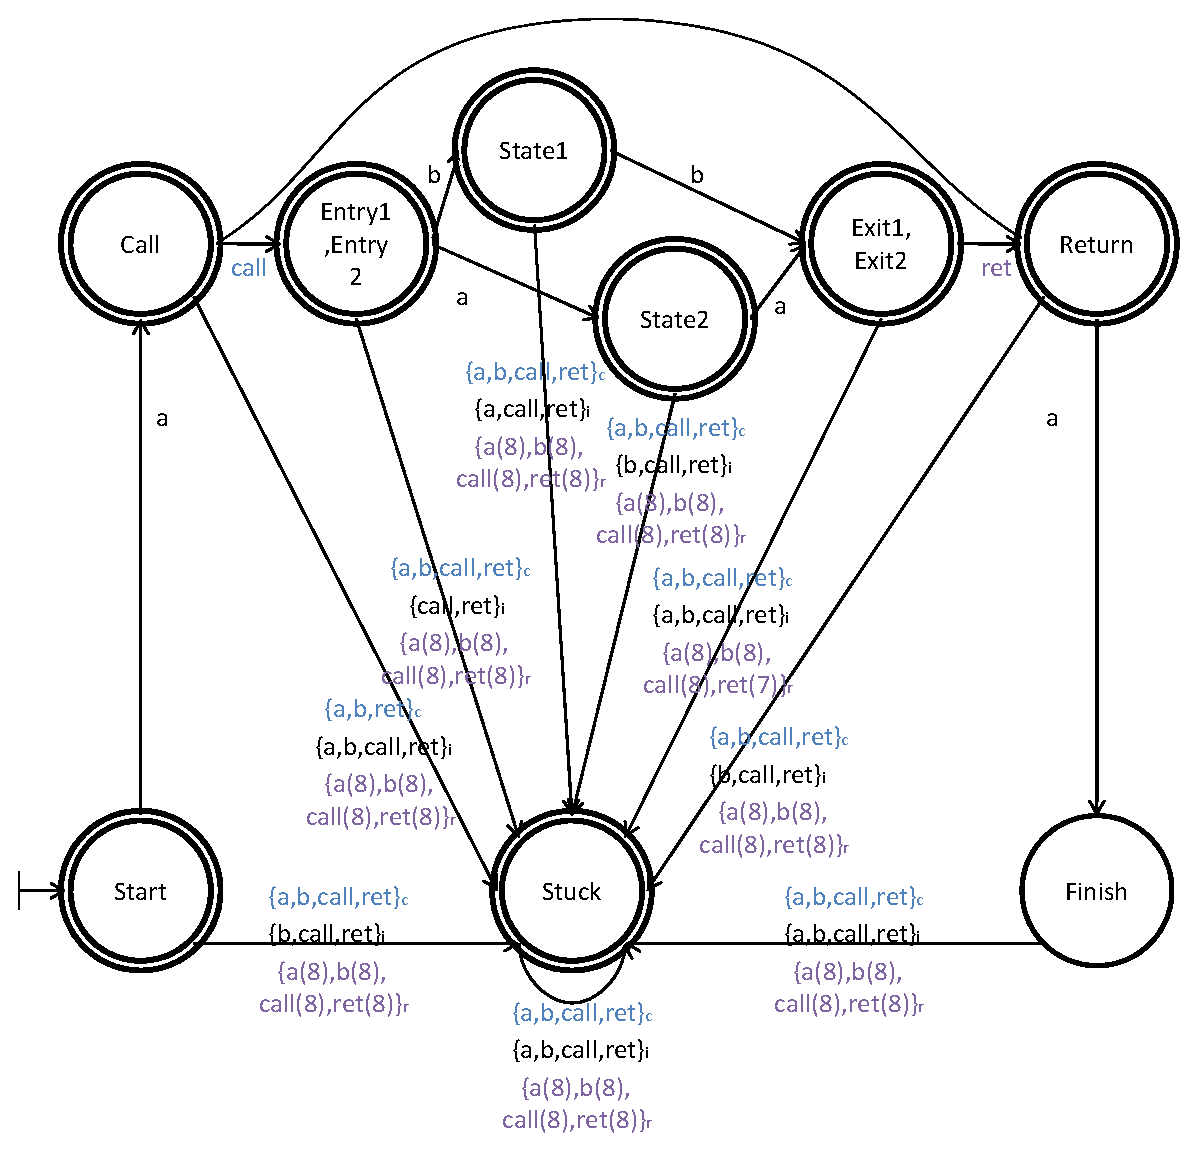
\includegraphics[width=12cm]{Figures/Figure20}
  \caption{The complement of the NWA in Figure \ref{Fig:Det1} (the
    determinization of which is shown in Figure \ref{Fig:Det2}).}
  \label{Fig:Comp1}
\end{figure}

Client information is copied directly
from the determinization of the original NWA using \texttt{ClientInfo::clone()}.


